\documentclass[border=10pt]{standalone}
\usepackage{xcolor}
\usepackage{tikz}

% Required TikZ libraries for advanced features
\usetikzlibrary{
    positioning,     % For relative node placement (e.g., below=of)
    shadings,        % For gradient fills in nodes
    arrows.meta,     % For customizable arrow tips (e.g., Stealth)
    calc,            % For coordinate calculations
    backgrounds      % To set a background color for the picture
}

% --- Color Definitions ---
% These colors are sampled from the original image for accuracy.
\definecolor{bgcolor}{HTML}{F0F2F8}
\definecolor{bordercolor}{HTML}{2C3A7A}
\definecolor{attention_left}{HTML}{D95B69}
\definecolor{attention_right}{HTML}{C7D2F2}
\definecolor{add_left}{HTML}{8A47AB}
\definecolor{add_right}{HTML}{E5394B}
\definecolor{conv_left}{HTML}{E1D9F3}
\definecolor{conv_right}{HTML}{C7D2F2}

\begin{document}

% The tikzpicture environment holds the entire diagram.
% The background is set using the 'backgrounds' library.
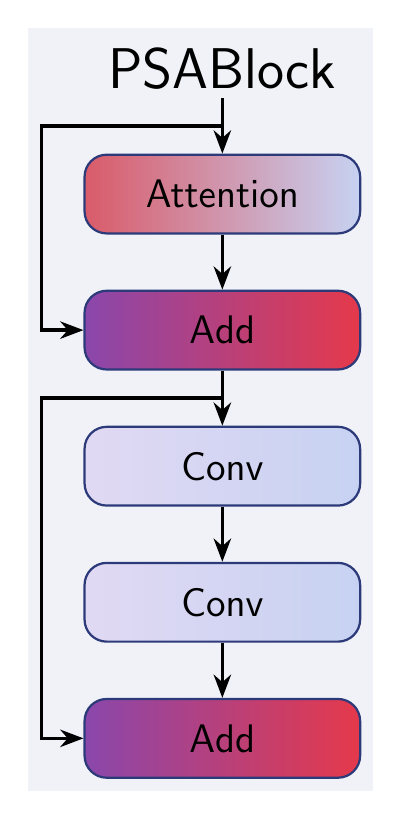
\begin{tikzpicture}[
    background rectangle/.style={fill=bgcolor}, 
    show background rectangle
]

    % --- Style Definitions ---
    % Using \tikzset for defining styles is modern and recommended.
    \tikzset{
        % A general style for all the main blocks in the diagram
        block/.style={
            rectangle, 
            rounded corners=8pt, 
            draw=bordercolor, 
            thick,
            minimum width=3.5cm, 
            minimum height=1cm,
            font=\sffamily\Large, 
            text=black,
            shade,           % Enables shading
            shading angle=0  % Makes the gradient horizontal (left to right)
        },
        % A style for all the arrows
        arrow/.style={
            ->, 
            very thick, 
            >=Stealth, % A common and clean arrow tip style
            black
        }
    }

    % --- Node Placement ---
    % Nodes are placed relative to each other for easy layout adjustments.
      %\node (c2psa) at (0, 8.5) {C2PSA};
    % The main title at the top
    \node[font=\sffamily\huge, text=black, yshift=-2.5cm] (title) {PSABlock};

    % The sequence of blocks, each with its specific gradient
    \node[block, left color=attention_left, right color=attention_right, 
          below=0.7cm of title] (attn) {Attention};

    \node[block, left color=add_left, right color=add_right, 
          below=0.7cm of attn] (add1) {Add};

    \node[block, left color=conv_left, right color=conv_right, 
          below=0.7cm of add1] (conv1) {Conv};

    \node[block, left color=conv_left, right color=conv_right, 
          below=0.7cm of conv1] (conv2) {Conv};

    \node[block, left color=add_left, right color=add_right, 
          below=0.7cm of conv2] (add2) {Add};

    % --- Drawing Connections ---
    
    % 1. Main vertical flow
    \draw[arrow] (title.south) -- (attn.north);
    \draw[arrow] (attn.south) -- (add1.north);
    \draw[arrow] (add1.south) -- (conv1.north);
    \draw[arrow] (conv1.south) -- (conv2.north);
    \draw[arrow] (conv2.south) -- (add2.north);

    % 2. Skip Connections (residual paths)
    
    % First skip connection from input to the first 'Add' block
    % A coordinate is placed on the path between title and attention block
    \coordinate (split1) at ($(title.south)!0.5!(attn.north)$);
    % The path is drawn by moving left, then down, then right into the node anchor.
    % The |- syntax helps create the orthogonal corners.
    \draw[arrow] (split1) -- ++(-2.3, 0) coordinate (c1) -- (c1 |- add1.west) -- (add1.west);

    % Second skip connection from the first 'Add' block to the second 'Add' block
    % A coordinate is placed on the path between the first add and first conv block
    \coordinate (split2) at ($(add1.south)!0.5!(conv1.north)$);
    % The same path drawing technique is used.
    \draw[arrow] (split2) -- ++(-2.3, 0) coordinate (c2) -- (c2 |- add2.west) -- (add2.west);

\end{tikzpicture}
\end{document}